\documentclass[12pt]{article}
\usepackage{amsmath}
\usepackage{graphicx,psfrag,epsf,float}
\graphicspath{C:/Users/Colin/Documents/GitHub/BB_data_analysis/paper}
\usepackage{enumerate}
\usepackage{natbib}
\usepackage{url} % not crucial - just used below for the URL

% math macros 
\newcommand{\ind}{\stackrel{ind.}{\sim}}
\newcommand{\op}{\operatorname}

\newcommand{\myequation}{\begin{equation}}
\newcommand{\myendequation}{\end{equation}}
\let\[\myequation
\let\]\myendequation


\pdfminorversion=4
% NOTE: To produce blinded version, replace "0" with "1" below.
\newcommand{\blind}{0}

% DON'T change margins - should be 1 inch all around.
\addtolength{\oddsidemargin}{-.5in}%
\addtolength{\evensidemargin}{-.5in}%
\addtolength{\textwidth}{1in}%
\addtolength{\textheight}{1.3in}%
\addtolength{\topmargin}{-.8in}%


\begin{document}

%\bibliographystyle{natbib}

\def\spacingset#1{\renewcommand{\baselinestretch}%
{#1}\small\normalsize} \spacingset{1}


%%%%%%%%%%%%%%%%%%%%%%%%%%%%%%%%%%%%%%%%%%%%%%%%%%%%%%%%%%%%%%%%%%%%%%%%%%%%%%

\if0\blind
{
  \title{\bf A Hierarchical Bayesian Approach for Modeling Infant-Mortality and Wearout Failure Modes}
  \author{Eric Mittman 1\thanks{
    The authors gratefully acknowledge Bill Meeker for his comments and suggestions}\hspace{.2cm}\\
    Department of Statistics, Iowa State University\\
    and \\
    Colin Lewis-Beck \\
    Department of Statistics, Iowa State University}
  \maketitle
} \fi

\if1\blind
{
  \bigskip
  \bigskip
  \bigskip
  \begin{center}
    {\LARGE\bf Title}
\end{center}
  \medskip
} \fi

\bigskip
\begin{abstract}
The text of your abstract.  100 or fewer words.
\end{abstract}

\noindent%
{\it Keywords:}  3 to 6 keywords, (don't reuse words appearing in title)
\vfill

\newpage
\spacingset{1.45} % DON'T change the spacing!
\section{Introduction}
Failure data for series systems may be collected at the system level by end-users interested only in the lifetime of the system. In the case of complex, high-reliability systems where cause of failure is not available, a model of failure which
\begin{enumerate}[a]
\item can be estimated from the observed data
\item is flexible enough to fit the observed data
\item relies on an approximation of the understood underlying process
\end{enumerate}
is desirable. We present a Bayesian, hierarchical modeling approach for grouped failure data. We demonstrate this approach with a large, heavily censored real data set with multiple right-censoring and left truncation times. We extend the generalized limited failure population model (GLFP) by \citet{chan}, which provides a generative model for failure times in a population with infant mortality. This model is an example of a bathtub distribution, exhibiting distinct early and late failure modes. The GLFP model assumes there are two causes of failure, one of which affects only a fraction of the population, and that the cause of failure is unobserved. We extend this model to grouped data and show that by borrowing information across groups we can achieve good model fits for almost all groups. By working with posterior samples, we can easily make inference on a wide range of quantities of interest while accounting for uncertainty.

\subsection{Background}
In engineering applications, a product can often fail due to one out of a set of possible malfunctioning components.  For example, a computer system can fail if the mother board, disc drive or power supply stop working.  Circuit boards (CB) can fail due to a manufacturing defect or later as a result of normal wearout.  The general name for such products is a series system where the lifetime of the product is the minimum failure time across $s$ different components or risks \citet{nelson}.  A common assumption in series systems is the time to failure for each risk, $s$, is statistically independent.  Thus, the overall reliability of a unit is modeled using the product rule across all $s$ risks.  Parameter estimation is straightforward if the cause of failure is known for each observation.  With engineering systems data, however, the exact cause of failure is frequently unknown or masked from the researcher.  \\

Previous papers have employed various data assumptions and methodologies to model masked lifetime failure data.  When modeling computer system failures Reiser et al. assumed the cause of failure for each observation came from a known subset of failure modes, and estimation was performed using a Bayesian approach \cite{reiser}.  Chan and Meeker labeled the cause of circuit board failures as infant mortality, unknown, or wearout based on the time of observed failures.  This helped identify parameters when using maximum likelihood (ML) estimation.  Extending Chan and Meeker's analysis, Basu et. al used a Bayesian analysis with informative priors to better identify early versus late failure modes without making any data assumptions \cite{basu}.  Berger and Sun introduced the Poly-Weibull distribution where cause of failure is the minimum of a several Weibull distributions \cite{berger}.  More recently, Ranjan et al. considered a competing risk model for infant mortality and wearout as a mixture of Weibull and exponential failure distributions \cite{ranjan}.  Treating the unknown failure modes as incomplete data, an expectation maximization algorithm with ML was used, in addition to Bayesian estimation.

\subsection{Motivation}
The goal of this paper is to model, and compare, the lifetime distribution of different hard drive brands using the GFLP lifetime model.  Product populations often contain a mixture of defective and non defective units.  The hazard function for this type of population is often described as a bathtub curve: the beginning of the curve corresponds to defective units failing early, followed by a constant hazard, and then and upswing as units fail from wearout.  Ignoring this hazard structure, which exists for series systems and computer disk drives, could lead to spurious inference when comparing the reliability of hard drive brand models \cite{chan}.  The general limited failure population model (GFLP) combines different failure time distributions to account for bending hazard functions; for example, one parametric model for defective units (infant mortality) and a second model for wearout \cite{chan}.  Unfortunately, as often the case with lifetime data, the true causes of failure for the hard drives are masked, which presents challenges for parameter identification: especially with sample sample sizes. One option is to combine all drive models and estiamte an overall GFLP model.  While this model can be precisely estimated, the data indicate a common model for all drive models fits well for only a few drive models.  At the other extreme, fitting individual models to each hard drive brand excludes drive brand models with one or two failures.  The GFLP model applied to these data produces very imprecise parameter estimates or can only be fit if highly informative priors are imposed.  Therefore, we propose to fit the GFLP model using a hierarchical Bayesian approach.  With over 60 brand drive models in testing a hierarchical model is advantageous as it pools information from across brands to get more precise estimates of individual drive model parameters.  Moreover, the hierarchical model is a nice compromise between the aggregate and individual modeling approaches: drive models with lots of failures can be estimated precisely; and in cases where little data is available the hierarchical model borrows information from other models to obtain stable estimates.  This allows us to include all of the hard drive data and more importantly, make reliability inference for all the drive models in the data set. 

\subsection{Overview}
The structure of the paper is as follows.  Section 1 summarizes the Backblaze data and the unique modeling challenges it presents.  Section 2 introduces the GFLP model as a mixture of two Weibull distributions.  In Section 3 we fit multiple specifications of the GFLP model to best describe the Backblaze data.  We also discuss computational and modeling issues that suggest a final model with a common Weibull distribution for defective units and individual Weibull distributions for the wearout failure mode.  In Section 4 we compare hard drive brand models based on our final GFLP model.  Finally, in Section 5, we review the GFLP model and propose future extensions.

\section{Data}
Backblaze is a company that offers backup storage to protect against hard drive failure.  While selling storage space is Backblaze's main business, since 2013 it has been collecting data on hard drives operating at its facility.  The purpose is to provide consumers and businesses with reliability information on different hard drive brands and models.  The hard drives continuously spin in controlled storage pods where they run until failure.  When a hard drive fails it is permanently removed, and new hard drives are regularly added to the storage pods.  In addition, the number of storage pods is increasing as Backblaze adds new hard drive brands to the sample.  Every quarter Backblaze makes its data publicly available through their website \cite{backblaze}. In addition, Backblaze publishes summary statistics of the different hard drive models currently operating.  No other analysis or modeling of the failure data is provided; however, Backblaze does encourage the public to further analyze its data, which for this paper goes through the first quarter of 2016.

As of the first quarter of 2016, Backblaze was collecting data on 63 different hard drive models.  Some drive models have been running since 2013, while others have been added at a later date.  There are a total of 75,297 hard drives running.  The distribution of drives by model varies: some models have only 1 drive in testing; the maximum number of drives running for a specific drive model is 35,860.  We can also look at the distribution of total number of failures and total time on test across all drive models.  As seen below, some drive models contain a lot of information, while others have few failures or a little time in operation. [INSERT FIGURE 1]. \\

Probability plotting is an effective method to check the adequacy of various parametric models to the data.  Identifying whether failure data follows a specific distribution is difficult to do by eye: especially when looking at pdfs or other non-linear plots.  However, if we can linearize the cumulative distribution function it is easier to visually assess a distributional goodness of fit; if a model is appropriate, a non parametric estimate of $\hat{F(t)}$ graphed on linarized probability scales should approximately follow a straight line. \\

For the hard drive data we first estimate the empirical cdf for each model using the Kaplan-Meier estimator \cite{kaplan}.  With left truncation, however, the Kaplan-Meier estimate, $\widehat{F(t)_{KM}}$, is conditional based on hard drive $i$ surviving up to time $\tau_i^L$ where $L$ is the amount of time the hard drive was running before Backblaze starting monitoring the drive.  To get the unconditional distribution we correct the non-parametric estimates using a parametric adjustment outlined by Turnbull, and given in more detail by Meeker and Escobar \cite{turnbull,meeker}.  For each hard drive model we select $\tau_{\text{min}}^L$, the smallest left truncated time in the sample.  Then, using the parametric estimates of the parameters, we calculate $Pr(T>\tau_\text{min}^L)$ the probability a hard drive has survived up to $\tau_{\text{min}}^L$.  We then apply this correction to the non parametric estimates, which results in the unconditional distribution of time to failure.\\

In Figure 2 we plot the Kaplan-Meier adjusted cdf for hard drive model X on Weibull paper.  Each point on the plot corresponds to a hard drive failure.  Censored drives are not plotted.  As mentioned in the introduction, the population of hard drives exhibits two primary failure modes.  One mode is a result of manufacturing defects, which cause early failures, known as infant mortality.  The second mode is non-defective hard drives that eventually fail due to wearout.   Evidence of at least two failure modes is seen in the Kaplan Meier plot with a kink occurring around hour Z.  Therefore, fitting a single Weibull model would not be flexible enough to model the failure distribution.


\section{Hierarchical GLFP model}
For modeling the lifetime of hard-drives, we select the Generalized Limited Failure Population model of \citet{chan}.
Let $T_{d,i}$ be the time of failure for the $i^{th}$ drive of drive-model $d$.
We assume that $T_{d,1},\ldots T_{d,n_d}$ are independent and have a probability distribution with cdf given by
$$P(T_{d,i}\le t) = 1 - (1-\pi_d\, F_{d1}(t))(1 - F_{d2}(t)), \mbox{ for }t>0 \mbox{, and where } \pi_d \mbox{ is in }(0,1).$$

As in \cite{chan}, we assume $F_{dj}$ is a member of the Weibull family of cdfs and parameterize in terms of a log-location parameter $\mu_{dj}$ and log-scale parameter $\sigma_{dj}$ so that

$$F_{dj}(t) = 1 - \exp \left\{ -\exp \left\{ \frac{ \log (t) - \mu_{dj}}{\sigma_{dj}} \right\} \right\},\; t>0, j=1,2$$

For the purpose of exposition, we will refer to the probability distributions $F_{d1}$ and $F_{d2}$ as ``failure modes." Specifically, we will refer to $F_{d1}$ as the ``early failure mode", and $F_{d2}$ as the ``main failure mode." The interpretation of the parameter $\pi_d$ is to represent the proportion of units susceptible to early failure, hence susceptible to both failure modes. Here the cause of failure is not assumed to be known, thus units of the same drive-model are exchangable.

To borrow strength across models, we can either share parameters across drive-models, or model the drive-model specific parameters hierarchically, allowing the data to inform the hyperparameters. For the second option, we model the scales, $\sigma_j$, quantiles, $t_{p_j,d,j} = \Phi^{-1}(\mu_j)$, and proportions, $\pi_d$, of the component distributions as follows:

$$\sigma_{d,1} \ind \op{Lognormal} \left( \eta_{\sigma,1}, \tau^2_{\sigma,1} \right) \mbox{ for } d=1,\ldots,D$$
$$\sigma_{d,2} \ind \op{Truncated-Lognormal} \left( \eta_{\sigma,2}, \tau^2_{\sigma,2} , 0, 1, \right) \mbox{ for } d=1,\ldots,D$$
$$t_{p_j,d,j} \equiv \mu_{d,j} + \sigma_{d,j}\,\Phi^{-1}(p_j)  \ind \op{Normal} \left(\eta_{t_{p_j},j}, \tau^2_{t_{p_j},j}\right) \mbox{ for } j=1,2\; d=1,\ldots,D$$

$$\op{logit} \pi_d \ind \op{N}(\eta_pi, \tau_pi) \mbox{ for } d=1,\ldots,D.$$

Here, $\Phi^{-1}$ is the quantile function of the standard log-Weibull distribution. We truncate $\sigma_{d,2}$ at $1$, appealing to the logic that wearout implies an increasing hazard function. The decision to parameterize in terms of a quantile other than the log-location parameter, $\mu = \Phi^{-1}(.5)$, is that lifetime data often features heavy right-censoring where inferences about the location parameter are extrapolations beyond the range of the data. For this data we selected $p_1=0.5,\mbox{ (the median), and } p_2 = 0.2$.

We consider the models with the following set of restrictions (from most to least restrictive):

\begin{enumerate}
\item $\pi_{d} = \pi,\quad \mu_{d1} = \mu_1,\quad \sigma_{d1}=\sigma_1,\quad \mu_{d2} = \mu_2,\quad \sigma_{d2} = \sigma_2$
\item $\pi_{d} = \pi,\quad \mu_{d1} = \mu_1,\quad \sigma_{d1}=\sigma_1,\quad \sigma_{d2} = \sigma_2$
\item $\pi_{d} = \pi,\quad \mu_{d1} = \mu_1,\quad \sigma_{d1}=\sigma_1$
\item $\mu_{d1} = \mu_1,\quad \sigma_{d1}=\sigma_1$
\end{enumerate}

The set of model specifications were chosen based on the data, interpretation of the model, as well as estimation considerations. Drive brand specific parameters for the the wearout failure mode $(\mu_{d2},\sigma_{d2})$, and the proportion defective $(\pi_d)$, are considered as a means to account for heterogeneity across brands in the right tails of the failure distribution.  Going from a common model for all hard drive brands and gradually increasing the complexity of the model, we end up at Model 4.  Model 4 allows for the probability of infant mortality as well as the shape and scale parameters for the 2nd failure mode to vary by brand drive model.

For all of the models we consider, the parameters for the infant mortality failure mode are held in common across drive brand models. We found that there was insufficient information in the data to model these parameters hierarchically.  Moreover, assuming a common distribution for infant mortality allows for straightforward interpretation of the quantities like $\frac{\pi_{d}}{\pi_{d'}}$. 

\subsection{Priors}
To complete the full probability model, we need to select prior distributions for the parameters governing the hierarchical model. We select proper priors to ensure a proper posterior. For the scale hyper-parameters we follow the recommendations of \citet{gelman2014bayesian} and use half-Cauchy priors. As for the location hyper-parameters, we select weakly informative priors consistent with our prior information on hard-drives. The prior for $\eta_\pi$ puts 95\% of prior mass on the interval $(0.006, 0.27)$ for the median proportion defective (What justification? Should maybe be lower.) For $\eta_{\sigma, 2}$, 95\% of prior mass is on values greater than $0.037$. Since $\sigma_d$ is the reciprocal of the Weibull shape parameter, this correponds roughly to an assumption that the median Weibull shape parameter is less than $1/0.037 = 27$. The prior for $\eta_{t_{p_2},2}$ implies that the median 20th percentile for non-defective units is less than greater than 3 days and less than 24 years.

\begin{align*}
  \eta_{\pi} & \sim \op{Normal}(-3, 1)\\
  \tau_{\pi} & \sim \op{Cauchy}^+(0, 1)\\
  \eta_{\sigma ,2} & \sim \op{Normal}(0, 2)\\
  \tau_{\sigma ,2} & \sim \op{Cauchy}^+(0, 1)\\
  \eta_{t_{.2_2},2} & \sim \op{Normal}(9, 2)\\
  \tau_{t_{.2_2},2} & \sim \op{Cauchy}^+(0, 1)
 \end{align*} 

\subsection{Computation}
Discuss the MCMC approach, RStan, etc.

\section{Data analysis}
\subsection{Results}
Show some of the fits of the GFLP Model.  Also present the unpooled output for a few models.  Show parameter estimates with uncertainty. 

\subsection{Model Comparisons}
First look at the overlaid posterior credible bands. \\

In addition to graphically examining model fits via posterior credible bands, we compared the predictive accuracy of the 4 different models using an approximate leave-one-out cross validation (LOO) method.  The predictive accuracy from a fitted Bayesian model can be estimated simply with posterior simulations of the model parameters \cite{vehtari}.  For each observation, $i$, the log point-wise predictive density is calculated over the full set of posterior parameters with the $i$th data point removed.  The final expected point-wise predictive density is the sum over all observations (elpd $=\sum{\log p(y_i|y_{-i})}$).  To obtain a more stable estimate of elpd, Vehtari et. al suggest using Pareto smoothed importance weights (PSIS) since the tail of the importance weights used to estimate elpd is often long.  We computed the elpd for all 4 models using the R package loo \cite{loopackage}.  When $n$ is large, the distribution of the elpd is approximately normal and models can be statistically compared.  We calculated the difference in expected predictive accuracy for all 4 models as well as the standard error of the difference.  As the model complexity increased, the predictive accuracy improved (Table 1).  Of all the models, Model 4 had the best predictive accuracy and was significantly better than models 1-3.

\subsection{Brand Comparisons}
Ideas for plots: A graph comparing the pi's for all drive models.

I think a graph looking at the B10 using the full model could be good, too.  Something like the graph below.  Perhaps we could sort drive model based on sample size?

\begin{figure}[H]
    \centering
   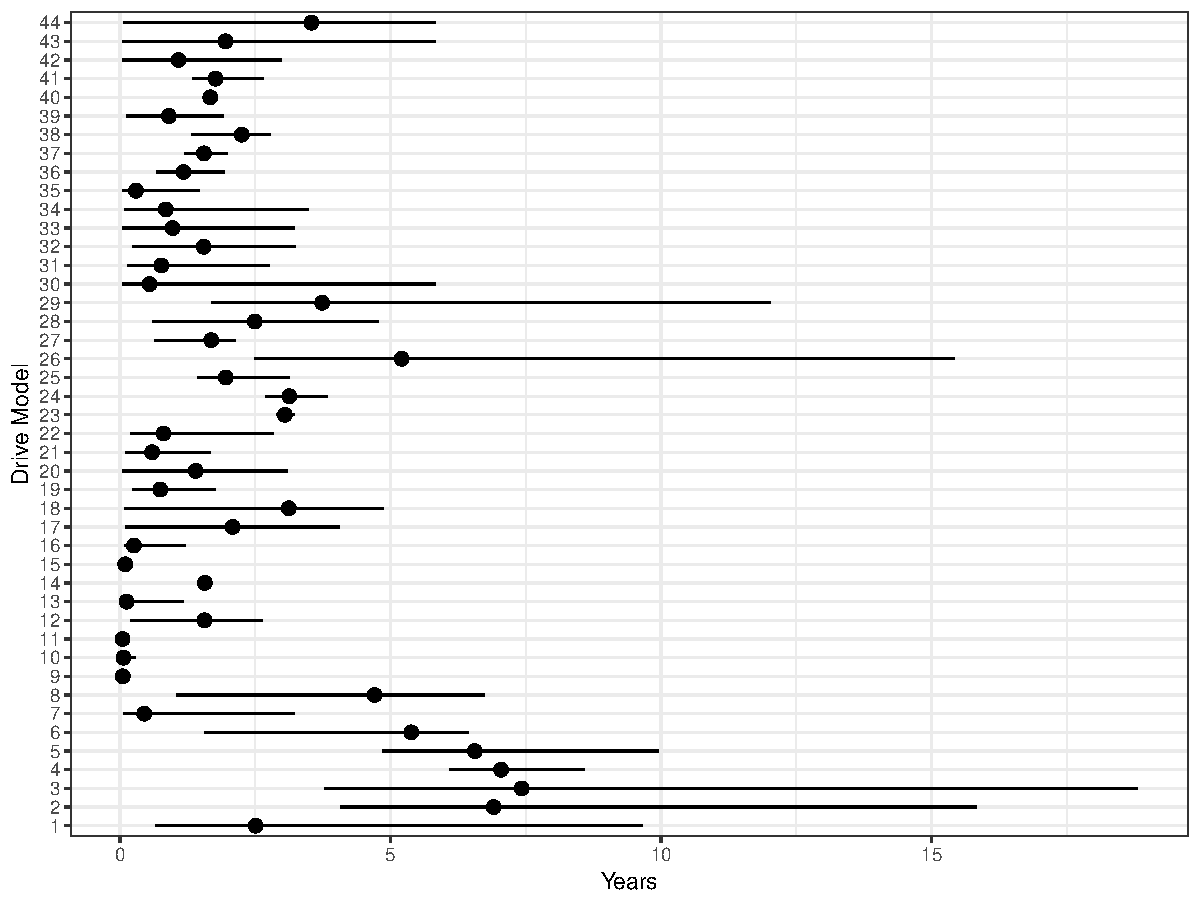
\includegraphics[width=6.0in]{B10_full.pdf}
		\caption{B10 in Years for All Drive Models \label{fig:first}} 
\end{figure}

\section{Concluding Remarks and Extensions}
Review the advantages of fitting the GFLP model and offer future ideas.  




    


\bigskip
\begin{center}
{\large\bf SUPPLEMENTARY MATERIAL}
\end{center}

\begin{description}

\item Put R Stan code here

\end{description}

\bibliographystyle{plainnat}
\bibliography{sample}

\end{document}
